%%%%%%%%%%%%%%%%%%%%%%%%%%%%%%%%%%%%%%%%%%%%%%%%%%%%%%%%%%%%%%%%%%%%%%%%% 
% $Id$
% %%%%%%%%%%%%%%%%%%%%%%%%%%%%%%%%%%%%%%%%%%%%%%%%%%%%%%%%%%%%%%%%%%%%%%%%%
%
% Set de slides nostrando los cambios relativos al postproceso que
% produce resultaods de near field para verlos en la interfaz.
%
% %%%%%%%%%%%%%%%%%%%%%%%%%%%%%%%%%%%%%%%%%%%%%%%%%%%%%%%%%%%%%%%%%%%%%%%%%

  
  \begin{frame}[allowframebreaks]{Postprocesssing  changes}{Extra information in
      nearfield}

    \begin{block}{Changes in nearfield postprocessing}
      \begin{itemize}
      \item Added a 3-character string after \texttt{surf} to denote
        the kind of boundary condition that surface is (DIR, NEU, NUL,
        ABC,\ldots)
      \item Added to the surface set the surfaces involved in FE-IIEE
        method, denoted as \texttt{fe-iiee-local-ext}, and
        \texttt{fe-iiee-local-int}, corresponding to $S$ and $S'$
        surfaces respectively.
      \end{itemize}

    \end{block}

    \framebreak % %%%%%%%%%%%%%%%%%%%%%%%%%%%%%%%%%%%%%%

    \begin{center}
      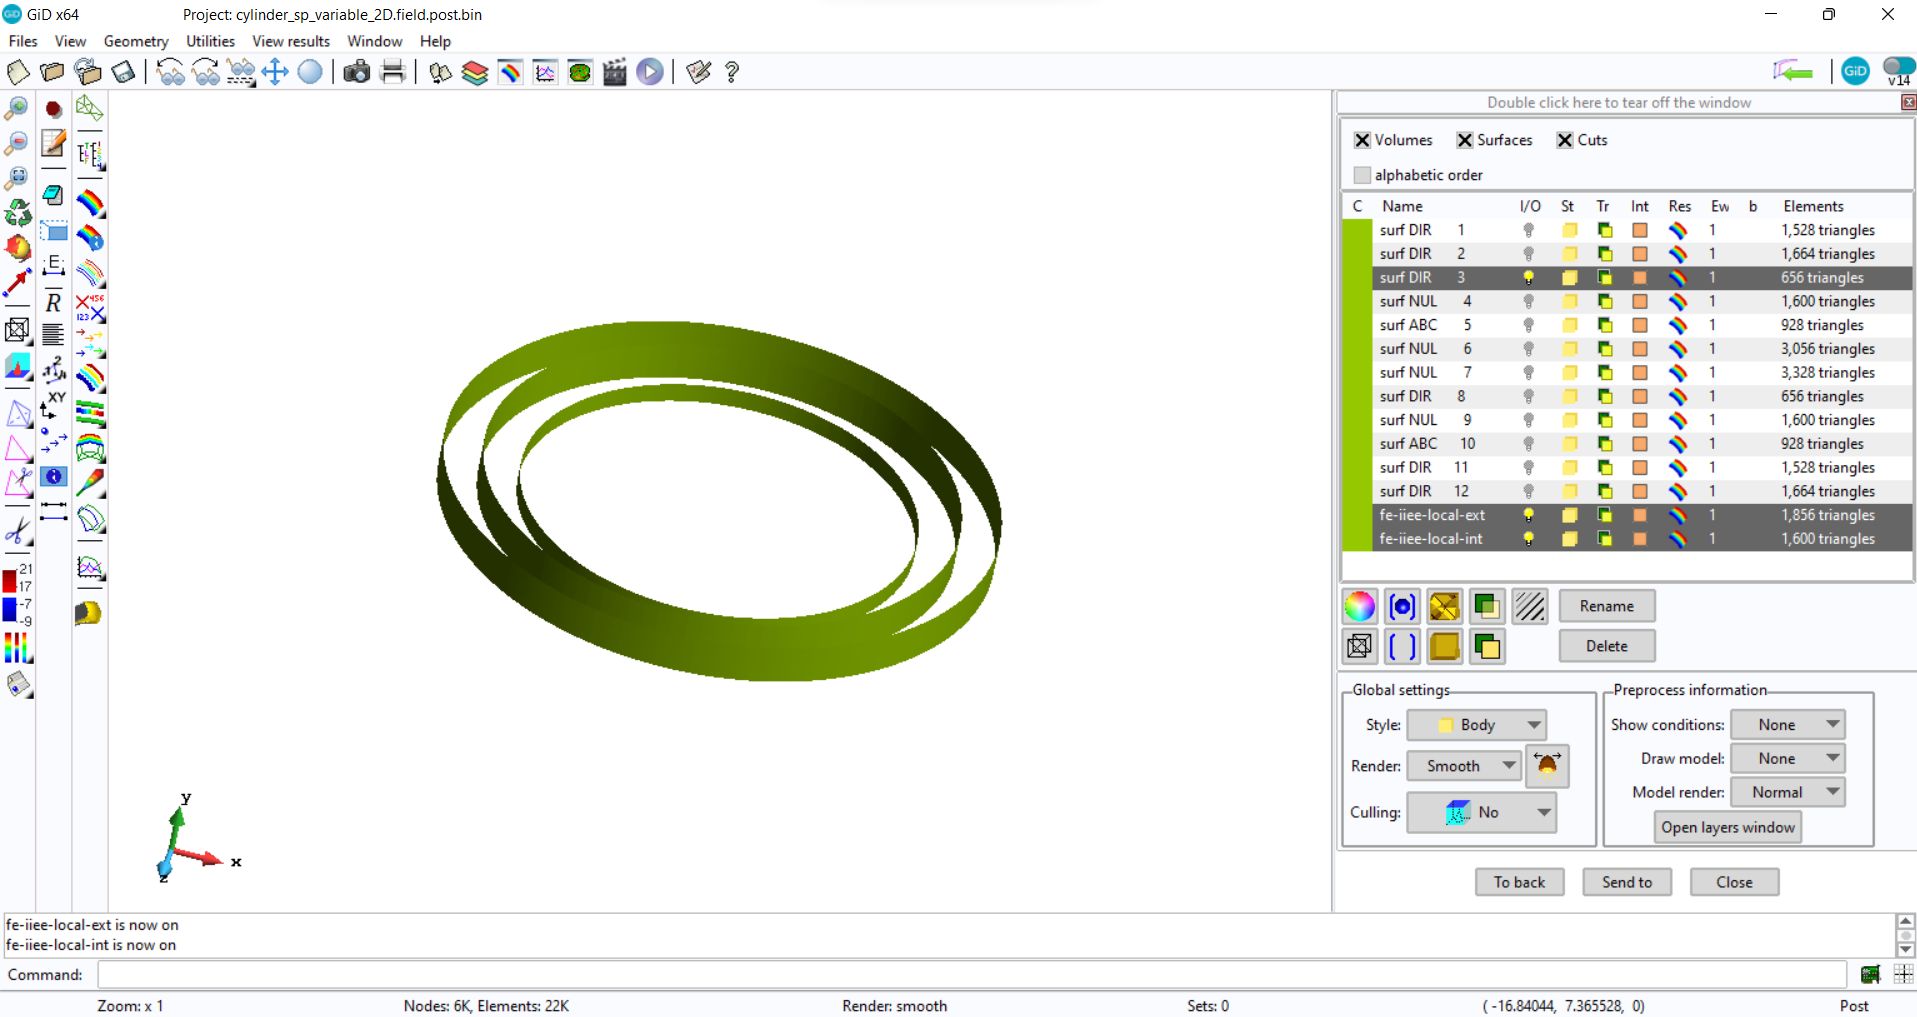
\includegraphics[width=\textwidth]{postprocessing_changes} 
    \end{center}

    
  \end{frame}

  % %%%%%%%%%%%%%%%%%%%%%%%%%%%%%%%%%%%%%%%%%%%%%%%%%%%%%%%%%%%%%%% 
  
  \begin{frame}[allowframebreaks]{Postprocesssing  changes}{Extra information in
      nearfield}

    \begin{columns}
      \column{0.48\textwidth} \centering
      {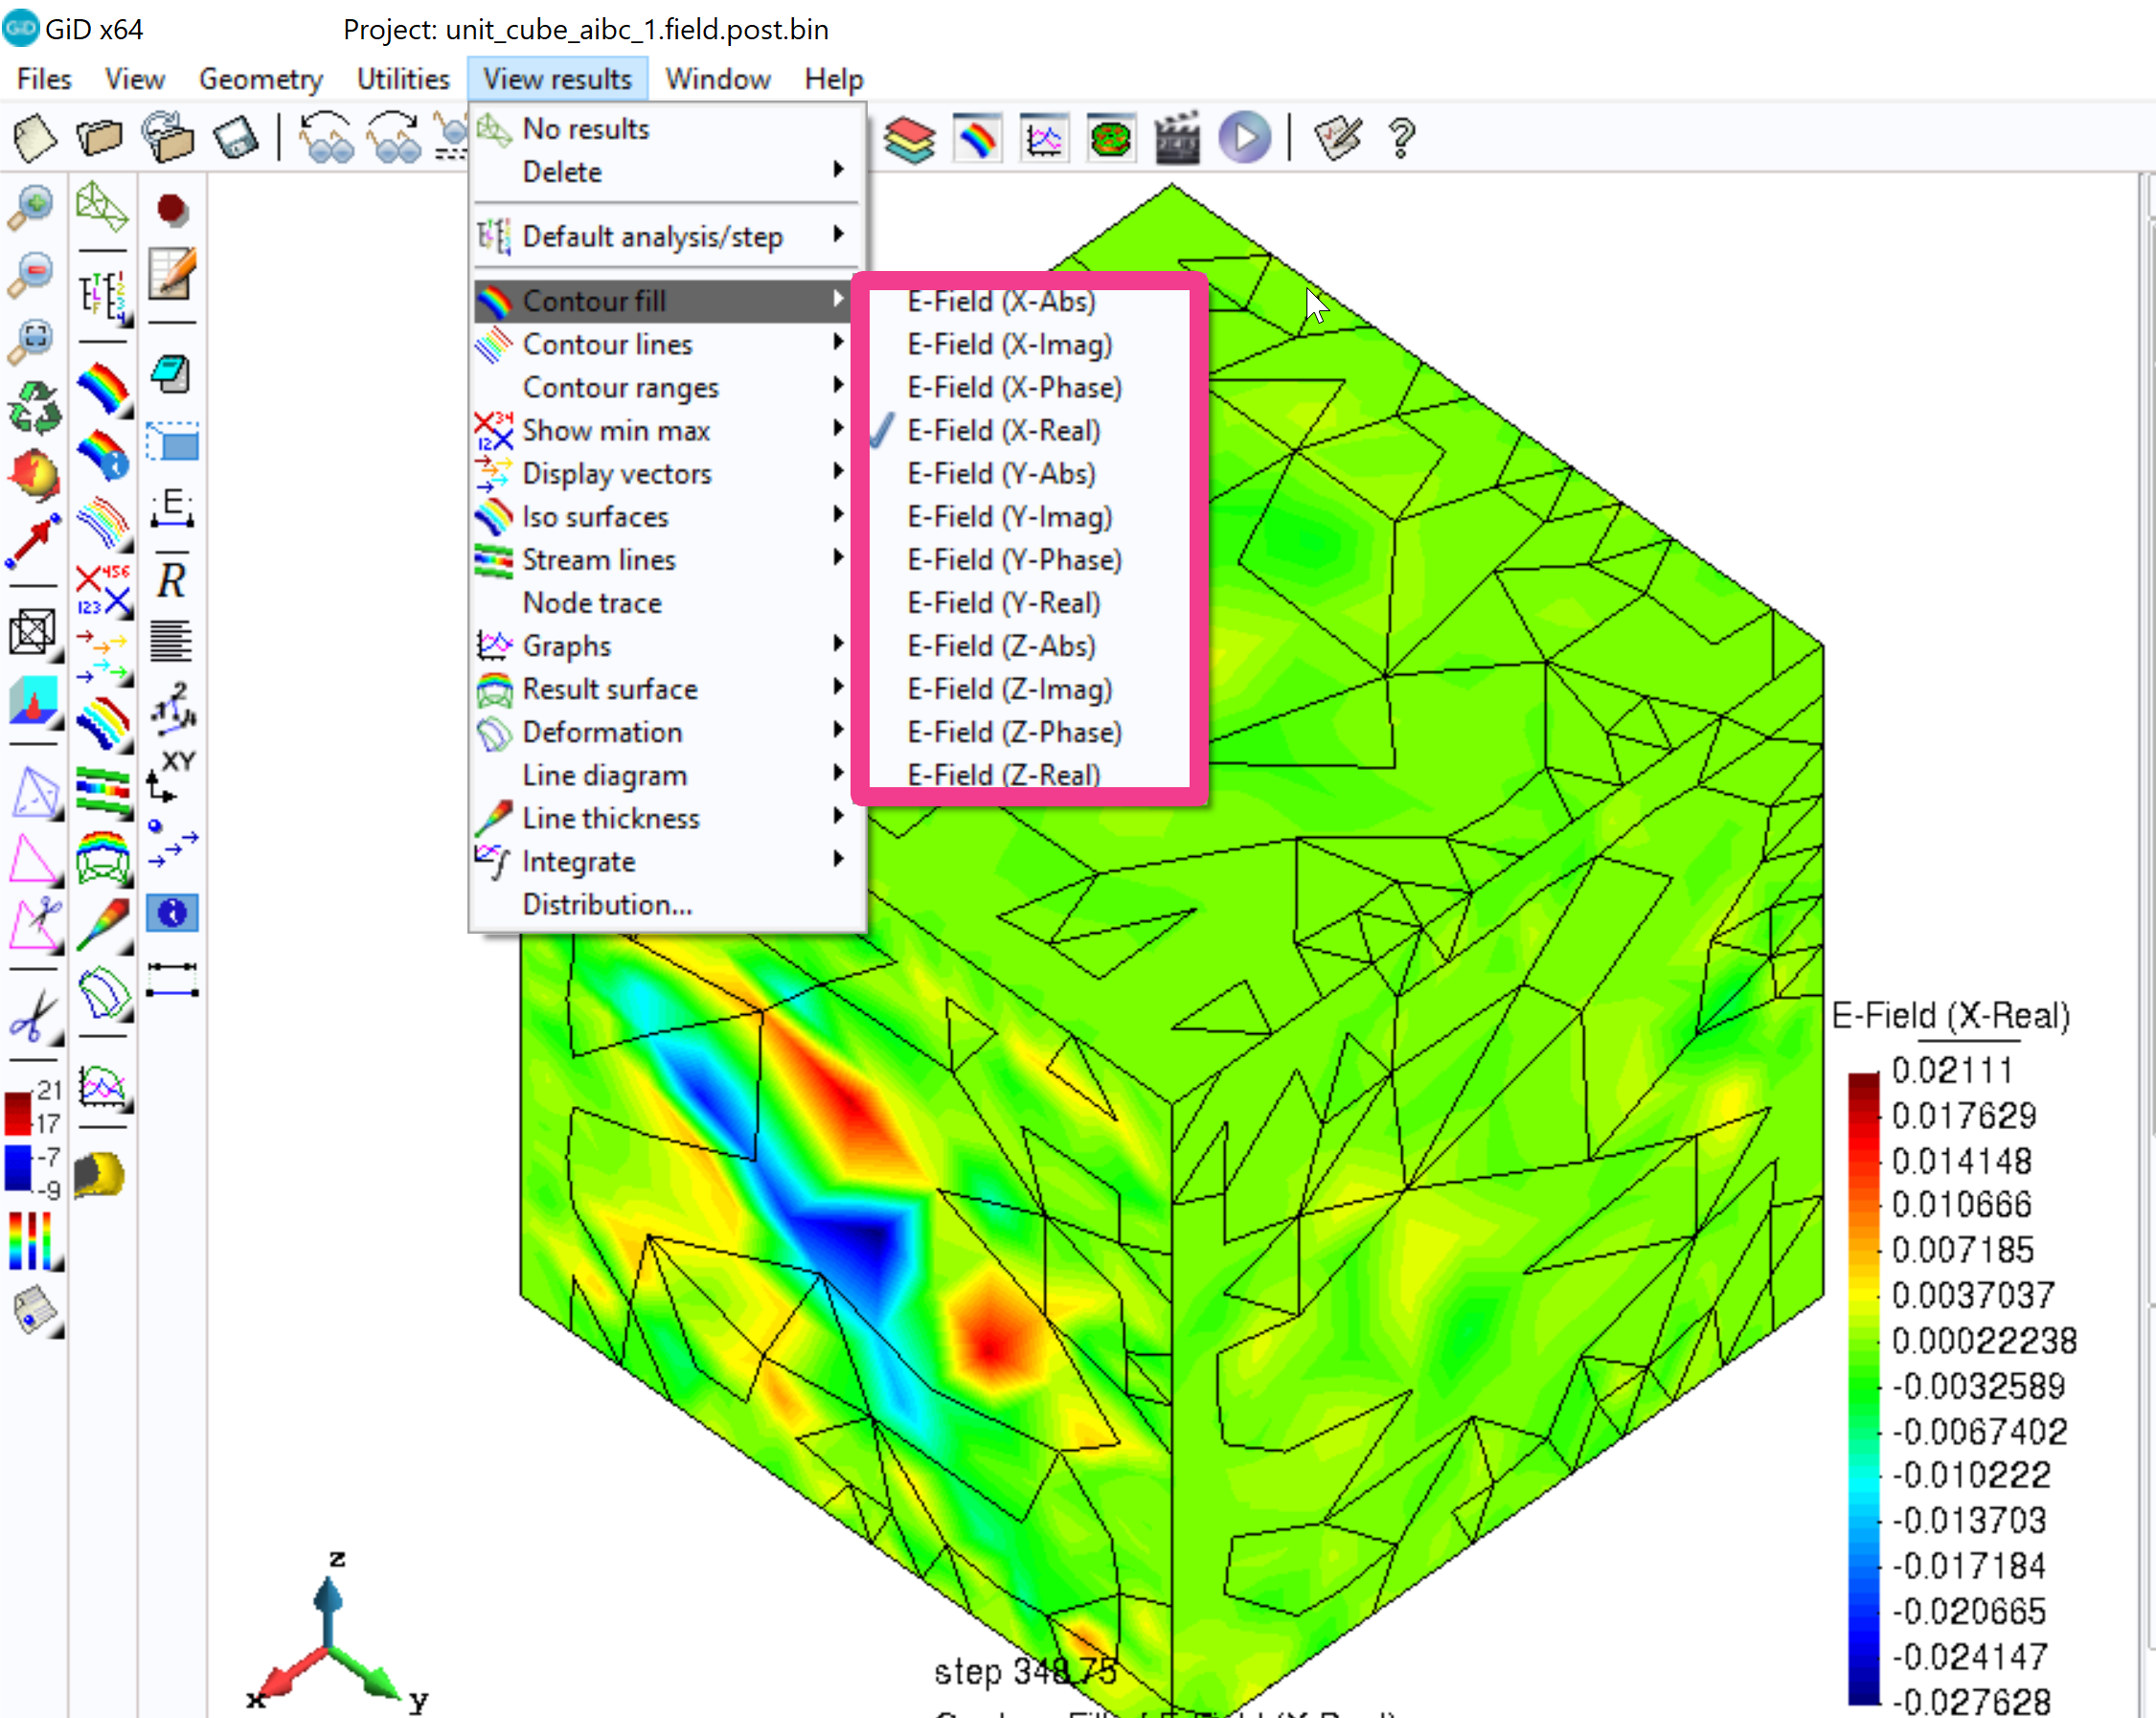
\includegraphics[angle=0,width=\textwidth]{hofem_new_postprocess.png}}
      \column{0.48\textwidth}
      {
        \begin{itemize}
        \item Included a new option to get all the available results for the 
          near field.
        \item Implemented as a new option called \texttt{all-xyz}.
        \end{itemize}
      }
    \end{columns}
    
  \end{frame}
    
    % %%%%%%%%%%%%%%%%%%%%%%%%%%%%%%%%%%%%%%%%%%%%%%%%%%%%%%%%%%%%%%%
